\section{Mechanische analysis}

Naast dat de testkast de motoren moet kunnen aansturen moeten de motoren ook op de montage plaat passen. Veel gaten hiervoor zitten er al op de montage plaat maar voor sommige motoren moeten er nog wel gaten worden geboord. Voor dit onderzoek is er onderzocht waar deze gaten moeten komen en deze zijn getekend in het 3D model (Solid Edge) dit zou dus alleen een kwestie van boren en tappen moeten zijn tijdens de implementatiefase.

\begin{figure}[H]
	\centering
	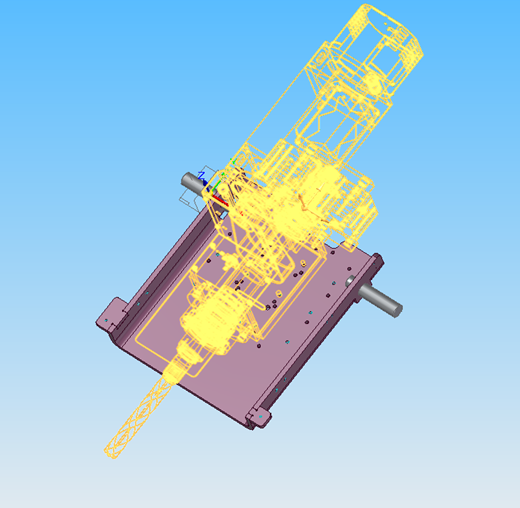
\includegraphics[width=0.6\linewidth]{Foto3Dmodel1}
	\label{fig:3Dmodel1}
	\caption{Voorbeeld gemonteerde motor 1}
\end{figure}

\begin{figure}[H]
	\centering
	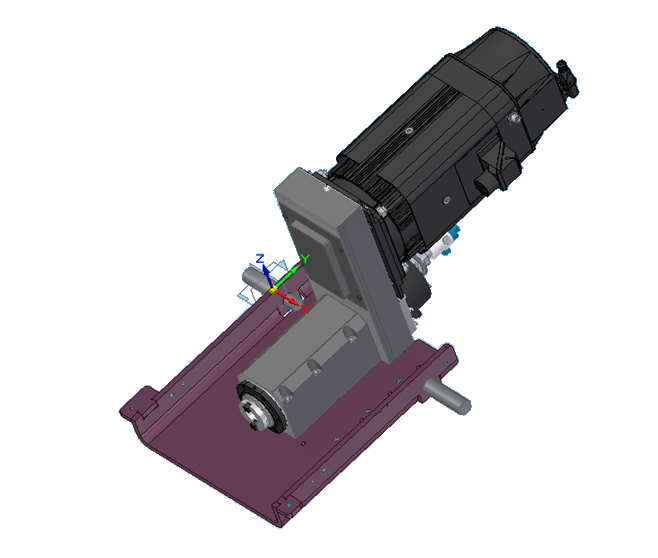
\includegraphics[width=0.6\linewidth]{Foto3Dmodel2}
	\label{fig:3Dmodel2}
	\caption{Voorbeeld gemonteerde motor 2}
\end{figure}